\chapter[VHDL]{Langages de description matérielle\\{\it L'exemple de VHDL}}
\minitoc

\section{Avant propos}
\lettrine{C}e chapitre est une introduction à VHDL. Ce langage sera étudié et utilisé plus en détail en deuxième année. Plusieurs
cours universitaires découplent totalement l'enseignement de l'Electronique numérique et celui de VHDL (ou Verilog). C'est une
démarche qui a du sens : elle permet notamment de raisonner sur les concepts de l'Electronique, avant de s'engouffrer dans les
particularismes de tel ou tel langage. Toutefois, notre expérience nous laisse penser qu'il est frustrant de s'arrêter si près
d'expériences possibles, simples et concrètes, qui permettent au futur ingénieur de mieux se projeter dans ce domaine passionnant
que sont les systèmes embarqués numériques. Nous avons donc choisi une {\it approche intermédiaire} qui consiste à se limiter à un survol
de VHDL, {\it restreint à cette seule UV 1.2 de l'ENSTA Bretagne}. Nous nous bornerons :

\begin{itemize}
  \item A la description de systèmes d'équations booléennes sous la forme d'{\it assignations concurrentes} de VHDL.
  \item A la description de bascule D sous la forme de {\it processus "clockés"}
  \item A la description de quelques bancs de test (testbench) qui illustrent la démarche de vérification par simulation.
\end{itemize}

Cette restriction laisse de côté les aspects les plus productifs de VHDL et notamment la maîtrise de la notion d'inférence au niveau transfert
de registres (RTL). Cela sera étudié de manière poussée en deuxième année. Les plus impatients pourront consulter différentes ouvrages \cite{chu_rtl}, \cite{chu_fpga}.
Dans les flots de conception traditionnels, notre restriction correspond stricto-sensu au niveau logique.

\section{Introduction : les langages de description matérielle}

\paragraph{Naissance de VHDL}

La Silicon Valley est née de l'essor qui a suivi l'invention du transistor (1947). Diverses sociétés concevant
des circuits à base de semi-conducteurs ont commencé à échanger des informations concernant la structure et le comportement temporel de circuits. On a rapidement compris
que les simples dessins ne suffisaient pas : la description des circuits requiert des langages spécifiques. Il s'agit des HDL ou "hardware description languages".
Au niveau analogique, c'est SPICE qui s'est imposé : il permet de décrire des assemblages de composants tels que des diodes, resistances, capacités, etc sous la forme d'une netlist textuelle.
Très rapidement, la nécessité d'un format commun de {\it description} des circuits numériques s'est également imposée. Le DARPA (Département à la Défense américain) a initié en 1981 la création
de VHDL. IBM, Intermetrics et Texas Instrument ont pris le projet en main. La syntaxe de VHDL s'est fortement inspirée d'ADA, un langage informatique généraliste et très prometteur à l'époque. C'est finalement en 1987 que l'IEEE publie un premier standard mondial,
amendé en 1993. Différentes évolutions ont eu lieu depuis, et des groupes de travail continuent de s'activer autour de l'évolution du langage. L'ambition du langage --initialement cantonné
à la description de circuits-- s'est étendue : il a été rapidement possible de simuler, puis de synthétiser des circuits décrits en VHDL. En parallèle, un autre langage aux buts similaires est né :  Verilog, inventé pour la simulation logique par la société Gateway Design Automation,
puis commercialisé par la société Cadence, qui reste un des leaders mondiaux de l'EDA (Electronic Design
Automation). Verilog est également un standard IEEE désormais. A noter que plus tard, d'autres langages de description matérielle ont vu le jour : on pense notamment à SystemC, qui élève le niveau d'abstraction
au dessus de ce qu'il est possible décrire en VHDL ou Verilog.
Ce domaine de la description et de la modélisation de systèmes numériques reste très actif : ces outils de simulation et de synthèse sont la clé de voûte de toute l'Industrie du Semiconducteur.

\paragraph{Particularités de VHDL : deux sémantiques}

VHDL est un langage très exigeant en terme de syntaxe, réputée verbeuse (mais explicite) mais également en terme de "sémantique" : outre le fait qu'il est fortement typé, il possède
en réalité 2 sémantiques très différentes en ce qui concerne le {\it temps}. D'une part, il sert à la simulation sur ordinateur : la signification d'un programme VHDL est donc imposée par ce simulateur, qui doit
représenter le parallélisme final du circuit à l'aide d'un algorithme séquentiel. D'autre part, il sert à la synthèse de circuits qui existeront in fine, sur silicium. Le concepteur
en VHDL doit donc en permanence "jongler" avec ce qui est limité à la simulation et ce qui devra subir le flot de synthèse. La prise en compte de cette dualité nécessite beaucoup d'expertise.

\paragraph{Démarche de modélisation}
Ecrire des programmes VHDL nécessite d'adhérer à une démarche de modélisation très différente de l'écriture de programmes traditionnels (Python, Java, C etc). Comme leur nom l'indique,
les HDL sont utiles à la {\it description} de circuits : il est inutile d'écrire des programmes VHDL en imaginant qu'il correspondront "par miracle" à une circuit. Il faut avoir à l'inverse
le circuit sur papier ou tout au moins bien en tête, avant de se lancer dans sa description. Le modèle séquentiel des langages cités précédemment laisse {\it peut-être} l'opportunité de
programmer "au fil de l'eau" : ce n'est pas le cas ici. Dans notre utilisation de VHDL dans cette UV, il s'agit d'abord d'obtenir les équations logiques, puis de les transcrire en VHDL.
Ce sera également le cas en deuxième année, mais on se situera à un niveau d'abstraction (RTL) plus confortable que ces simples équations logiques : il existe des construction du langage
qui nosu affranchissent de l'écriture explicite des équations. Mais nous respectons ici le partie-pris pédagogique de restriction du langage.


% \section{Aperçu du flot de conception}
% \paragraph{Processus}
% Le {\it flot de conception} est le processus qui organise la création des systèmes numériques, mais aussi de leur vérification. Ce processus
% enchaîne un grand nombre d'étapes que nous nous sommes efforcés de simplifier ici. Chaque étape s'accompagne de ses propres techniques, outils et langages.
% Ces flots commencent très en amont, avec par exemple des réflexions en terme de marketing (quel est le besoin du marché, etc). On dégage de ces réflexions des spécifications de plus en plus précises.
% Ces spécifications peuvent être d'ordre algorithmique (fonctionnelles) ou englober des spécifications dites {\it non-fonctionnelles} : par exemple les dimensions
% de la future puce, sa consommation, sa compatibilité électromagnétique, etc. Ces spécifications aboutissent généralement à un plan
% d'ensemble de ces fonctions, interconnectées par des canaux de communications. Les langages comme VHDL peuvent intervir dès ces phases amont, jusqu'à des phases
% très avancées de réalisation. Ces canaux peuvent être plus ou moins
% abstraits, c'est-à-dire dont le détail n'est pas encore à portée de main.
% L'ingénieur cherche à rendre ces spécifications {\it exécutables}. Il cherche par là à s'assurer au plus tôt, par simulation,
% que l'ensemble du futur système répond aux exigences initiales. Ce modèle du système encore abstrait s'appelle un {\it prototype virtuel}.
% Toutefois, force est de constater que  l'ingénieur cherche
% généralement à se reposer au plus tôt sur des standards de communications entre fonctions : il s'agit de bus connus comme AMBA, AXI, Wishbone,etc.
% Il fait le plus souvent office, pour le flot aval, de {\it modèle de référence}, aussi appelé en anglais "golden model". C'est un modèle qu'on ne remettra
% guère en cause et qui permettra de {\it vérifier} que le comportement du circuit final (ou de tout intermédiaire) à bien le comportement
% attendu aux entrées-sorties.
%
% \paragraph{Testbenches}
% C'est par simulation que la vérification précédente s'effectue. Pour simuler un système numérique, il faut imaginer une véritable "paillasse" de
% laboratoire : ce laboratoire est également virtuel, dans le sens où les instruments n'existent pas physiquement, mais sont simulés. Par exemple,
% il sera nécessaire de simuler l'existence d'un générateur d'horloge ou autres générateurs de signaux spécifiques. De même, on devra
% brancher des sondes également virtuelles, des oscilloscopes, et des générateurs de fichiers. Dans le flot basé sur VHDL, tous
% ces "instruments" sont en réalité des composants VHDL plus ou moins abstraits. Nous verrons quelques exemples de tels codes.

\section{La structure globale d'un programme VHDL}

Les programmes que nous allons écrire présentent une structure systématique :
\begin{enumerate}
  \item Déclaration de \textbf{librairies} et de \textbf{packages} utilisés
  \item \textbf{Entity} : c'est la description des entrées-sorties du circuit, et de paramètres génériques éventuels (taille des données etc).
  \item \textbf{Architecture} : description de l'organisation interne du circuit.
\end{enumerate}
Ces déclarations apparaissent généralement dans cet ordre, dans un seul et même fichier. Notons que ce n'est toutefois pas une obligation : par exemple, une entité et son architecture
peuvent être décrites dans des fichiers séparés. Il s'agit d'{\it unités de compilation} : le compilateur VHDL est capable de les compiler individuellement et de les assembler au final.

\subsection{Déclaration de librairies et packages}
Un exemple est donné ici. Il fait appel à deux librairies fournies par l'IEEE. Ces librairies sont incontournables.
\begin{itemize}
  \item La librairie \textbf{std\_logic\_1164} permet d'utiliser les types les plus standard de VHDL, à savoir le type std\_logic et le type std\_logic\_vector.
  Ce sont simplement l'incarnation du "bit" et d'un ensemble de bits, mais cette librairie permet de bénéficier d'autres valeurs que '0' et '1'. Ces autres valeurs sont d'une grande aide lors de la simulation du circuit et
  permettent de trouver au plus tôt des cas litigieux.
  En pratique, il est par exemple intéressant de pouvoir savoir si un fil est effectivement piloté ou non par une tension : dans le cas où aucune tension ne pilote le fil,
  on affaire à une tension 'u' (unknown). Cette valeur apparait en simulation lorsque le concepteur a oublié de connecter ("driver") le fil (signal) concerné. De même, le concepteur
  a peut-être connecté deux sources sur un même fil :  ce dernier est alors en conflit (valeur 'x'). Ce dernier cas survient lorsque deux ou plusieurs sources tentent d'imposer leur tension. De même une équipotentielle peut se trouver dans un état de haute impédance (valeur 'z').
  Le type bit existe nativement (sans appel à des librairies) dans VHDL, mais n'est guère utilisé, car il a la faucheuse tendance de masquer les non-connexions précédentes ou les conflits.
 \item  La librairie \textbf{numeric\_std} : c'est la librairie qui nous permet entre autre de faire des calculs sur des nombres signés ou non signés. Le type std\_logic\_vector précédent
 n'autorise pas d'emblée ce type de calculs arithmétiques (c'est un tableau sans arithmétique associée). Un ensemble de conversions très utiles sont également disponibles dans cette librairie.
\end{itemize}

\lstset{basicstyle=\small,language=VHDL}
\begin{lstlisting}[frame=single]
  librairie ieee;
  use ieee.std_logic_1164.all;
  use ieee.numeric_std.all;
\end{lstlisting}


\subsection{Notion d'entité}
L'entité permet de décrire les \textbf{ports} d'entrées-sorties du circuit, ainsi que d'éventuels paramètres dit "génériques". C'est l'\textbf{enveloppe extérieure} du composant.
Pour être correctement utilisée, cette entité devra être instanciée en respectant ces entrées-sorties : il faudra venir connecter des \textbf{signaux} à ces ports.

Un premier exemple de description d'entité est donné ici, sans paramètre.
\lstset{language=VHDL}
\begin{lstlisting}[frame=single]
  entity example1 is
     port(
       reset_n      : in  std_logic;
       clk          : in  std_logic;
       a            : in  std_logic;
       b,c,d        : in  std_logic;
       data1,data2  : in  std_logic_vector(31 downto 0);
       data3,data3  : in  unsigned(7 downto 0);
       f            : out std_logic;
       dataout      : out std_logic_vector(15 downto 0)
     );
  end entity;
\end{lstlisting}
Cette entité présente un \textbf{nom} ("example1"), puis un ensemble de \textbf{ports}, qui sont des entrées ("in") ou des sorties ("out"). Notons qu'il existe aussi
le moyen de décrire des ports bidirectionnels ("inout"), qui ne seront pas décrits ni utilisés ici ; ils nécessitent des buffers trois-états. On remarque immédiatement
la syntaxe exigeante de VHDL, avec la présence de nombreuses parenthèses, signes de ponctuations (";",",")  et certaines redondances dans l'utilisation des mots clés ("entity").
Les bons éditeurs de textes comme Emacs fournissent une aide substantielle dans l'écriture du VHDL, en offrant des auto-complétions puissantes, voire la génération de gabarits (squelettes de
code ) complets, déclenchées sur des racourcis claviers.

\subsection{Notion d'architecture}
L'architecture est le contenu réel du circuit. Si l'entité était un capot de voiture, l'architecture représente le moteur, sous le capot.
Une architecture est explicitement associée à une entité unique. Notons par contre qu'une entité peut être associée à plusieurs architectures : cela restitue l'idée que derrière l'apparence externe d'un composant (derrière l'entité), on peut
trouver plusieurs organisations différentes, de la même manière que derrière un capot de voiture de course, on peut trouver soit un moteur performant, soit un un moteur plus banal etc.

\begin{lstlisting}[frame=single]
  architecture logique of example1 is
    -- ici les declarations necessaires a l'architecture :
    -- ...signaux notamment.
    signal w1 : std_logic;
    -- etc...
  begin
    -- ici le contenu effectif
  end logique;
\end{lstlisting}

Dans l'exemple donné, le nom de l'architecture est "logique" (choix évidemment libre), et le nom de l'entité associée est "example1".
L'architecture est elle-même structurée : une première partie permet de placer les déclarations locales à l'architecture. Le corps véritable de l'architecture se
situe entre les mots clés "begin" et "end". Noter que le "end" est suivi du nom de l'architecture.

\section{Les éléments clés de l'architecture}
C'est dans le corps de cette architecture que le concepteur peut réelement décrire son circuit en détail. Plusieurs nouveaux concepts sont mis à disposition, associés
à des éléments de syntaxe que nous allons détailler. La chose importante à comprendre est qu'au sein de cette architecture, l'ordre d'écriture de ces concepts
n'a pas d'importance : ceci diffère de ce que vous avez l'habitude d'écrire (python, java, etc). Ceci restitue pourtant naturellement l'idée de {\it décrire} le circuit
(imaginé, dessiné ou plus rarement existant), à la manière d'un naturaliste qui décrirait un fleur en se laissant le droit de commencer par la tige, les racines ou les pétales.
\subsection{Assignations concurrentes des signaux}

Les assignations concurrentes s'effectuent sur des {\it signaux} : une assignation est la manière d'affecter un signal. Un signal peut être vu comme un fil (une équipotentielle).
Les assignations s'effectuent en {\it parallèle} : en conséquence, un ensemble d'assignations concurrentes peuvent être vues comme un ensemble de définitions d'équations. Leur ordre n'a pas d'importance, ce qui
tranche avec la notion d'assignation de variable dans un programme impératif classique. Dans l'exemple
qui suit, la partie de droite de 'affectation du signal $w1$ est une expression booléenne. Dans la seconde assignation, la partie droite est plus complexe car elle est conditionnelle, mais in fine,
le synthétiseur logique synthétisera 8 équations logiques (une pour chaque fil du signal $w2$), après avoir {\it inféré} un réseau booléen constitué d'un additionneur, d'un multiplieur 8 bits et de multiplexeurs.

\begin{lstlisting}[frame=single]
  architecture logique of example1 is
    signal w1 : std_logic;
    signal w2 : unsigned(7 downto 0);
  begin
    -- ici deux assignations concurrentes

    w1 <= (a or b) and c;

    w2 <= (a+b) when cmd="00" else
          (a*b) when cmd="01" else
          to_unsigned(0,32);

  end logique;
\end{lstlisting}

\subsection{Processus}
Une autre manière d'effectuer des actions parallèles, qui figure dans le corps d'une architecture, est le recours aux {\it processus}. Un processus est un "bout de code", évalué de manière séquentielle par le simulateur.
Vous pouvez ainsi décrire des "programmes" séquentiels qui s'exécutent en parallèle et interagissent : leur moyen d'interagir est d'affecter des signaux. Le signal peut être vue comme des canaux de communication entre processus.
Une des grandes difficultés de VHDL est que ces processus, {\it évalués} de manière séquentielle par le simulateur, peuvent être utilisés à la description de dispositifs électroniques qui ne sont pas forcément séquentiels.
Ainsi, selon l'écriture, un processus résultera, après traitement par le synthétiseur, en un circuit combinatoire ou séquentiel. Etudions quelques exemples, afin de nous permettre d'y voir plus clair.

% BUG for ! : without escaping !!!!!!!!!!!!!!!!!!!!!!!!!!!!!!
\paragraph{Exemple 1 \: processus générant un circuit combinatoire}
Nous allons décrire le même circuit que précédemment, à l'aide d'un seul processus.

\begin{lstlisting}[frame=single]
 p1 : process(a,b,c)
 begin
   w1 <= (a or b) and c;
   w2 <= 1;
 end process;
\end{lstlisting}

Il s'agit  du même exemple que précédemment codé avec des assignations concurrentes. Le concepteur a la choix de la forme
qu'il utilise pour décrire son futur circuit. Ce processus (précédé d'un label optionnel --ici "p1"--), est structuré comme un programme séquentiel : chaque instruction du processus est d'ailleurs suivi d'un ";", marqueur traditionnel de séquentialité
dans les langages comme C ou Java. On y retrouve un "if"..."elsif". Le simulateur (lui-même séquentiel) profitera de cette forme séquentielle pour simuler aisément le circuit ; le simulateur calcule par contre
qu'aucun temps physique significatif ne s'est ici écoulé entre les instructions au début du processus et celles de la fin. Le synthétiseur, quant à lui, est capable d'inférer un matériel parfaitement combinatoire.
Ces deux manières de voir le processus sont ainsi cohérentes.

\paragraph{Exemple 2 \: processus générant un circuit séquentiel}
Exemple :
\begin{lstlisting}[frame=single]
architecture ex2 of circuit is
  signal d1,d2,q : std_logic;
begin
  p1 : process(clk)
  begin
    if rising_edge(clk) then
      q1 <= a;
    end if;
  end process;

  p2 : process(reset_n,clk)
  begin
    if reset_n='0' then
     q2 <= "000";
    elsif rising_edge(clk) then
      if enable='1' then
        q2 <= b;
      end if;
    end if;
  end process;

end logique;
\end{lstlisting}

Dans cet exemple, le concepteur a cherché à décrire deux bascules D, à l'aide de 2 processus. Le {\it principe fondamental} pour comprendre l'inférence de bascules D est le suivant :
\begin{center}
  \fbox{\begin{minipage}{0.9\textwidth}
     \textbf{Toute assignation d'un signal, sous la condition d'un front d'horloge, résulte en une bascule D}.
  \end{minipage}}
\end{center}


\paragraph{Exemple 3 : processus utilisé en banc de test}
Les processus sont également utilisés pour simuler des environnement de tests : ils peuvent décrire des générateurs de signaux, ou à l'inverse des instruments d'observation de signaux. Ces
processus ne servent que dans des {\it bancs de test virtuels} (testbench) sur lesquels nous allons revenir. Ces processus n'ont pas alors vocation à être synthétisable, et l'on peut donc
utiliser pleinement le langage VHDL. On qualifiera ces processus de "comportementaux".

Dans l'exemple suivant, on décrit la génération d'un signal (ou "stimulus"), à l'aide d'une processus qui opère sur plusieurs cycles d'horloge

\begin{center}
   \begin{minipage}[t]{9cm}
     \vspace{0pt}
     \begin{lstlisting}[frame=single]
     architecture bhv of circuit is
       signal s : unsigned(7 downto 0);
     begin
       stimulus : process(clk)
       begin
         s <=x"00";
         report "waiting for reset";
         wait until reset_n='1';
         for i in 0 to 10 loops
           wait until rising_edge(clk);
         end loop;
         report "starting sequence";
         s <= x"0A";
         wait until rising_edge(clk);
         s <= x"0B";
         wait until rising_edge(clk);
         s <= x"0C";
         wait until rising_edge(clk);
         s <= x"00";
         report "done."
         wait; --forever
       end process;

       -- autres processus ...

     end logique;
     \end{lstlisting}
  \end{minipage}%
  \begin{minipage}[t]{6cm}
   \vspace{40pt}
   \centering
   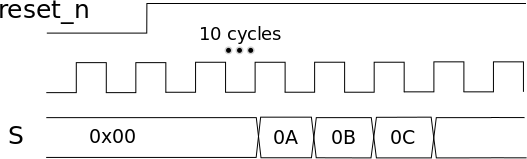
\includegraphics[width=5cm]{./figures/chronogramme.png}
  \end{minipage}
  \end{center} % added ending }
\subsection{Instanciation de composants et d'entités}
L'instanciation consiste à utiliser un modèle de circuit, précédemment décrit. Sans cette instanciation, un couple entité-architecture ne peut être simulé : il n'est pas "incarné", mais reste un modèle imaginé.
Une analogie naturelle peut être faite avec la programmation orientée objet, qui distingue bien la notion de {\it classe} et d'{\it objets} (appelés "instances"). Il faut dans notre cas imaginer
que l'on dispose d'une réserve infinie de composants sur étagère,et que l'on vient construire un système en les "posant" sur une table imaginaire. Cette table imaginaire est l'architecture associée à une entité :
l'instanciation se fait donc en parallèle des assginations concurrents vues précédemment. Elle permet en outre de construire des circuits hiérarchiques, à la manière des poupées russes (ou poupées gigognes) : un composant
peut être composé de composants etc...

Deux formes d'instanciations sont possibles : l'instanciation de {\it component} et l'instanciation d'{\it entity}. Une fois posés, ces composants devront être connectés aux signaux
en présence : horloge, reset, entrées, sorties, signaux locaux. Cette connection s'appelle le "port map". Comme nous allons le voir, il existe là aussi deux formes de port map : explicite ou positionnel.

\paragraph{Instanciation de composants}
La première forme a tendance a disparaître des pratiques, car elle requière notamment plus de texte : au sein de l'architecture receptacle, il est nécessaire de rappeler l'interface de l'entité, sous la forme
d'un "component". Supposons que l'on dispose d'un modèle entité-architecture d'un circuit "PGCD", dans un fichier "pgcd.vhd". Pour instancier ce circuit, il est nécessaire de procéder comme suit explicité dans
l'exemple.

\begin{lstlisting}[frame=single]
architecture bhv of circuit is

  component MonCircuit is
    port(
      reset_n      : in  std_logic;
      clk          : in  std_logic;
      a,b          : in  std_logic_vector(31 downto 0);
      f            : out std_logic_vector(31 downto 0);
    );
  end component;

  signal aa,bb, f1,f2 : std_logic_vector(31 downto 0);

begin -- instanciation de 2 composants

  -- port map explicite, de la forme :
  --    port formel => signal
  inst_1: MonCircuit
    port map (
      reset_n => reset_n,
      clk     => clk,
      a       => aa,
      b       => bb,
      f       => f1
    );

  -- port map positionnel
  inst_2: MonCircuit
    port map (reset_n,clk,aa,bb,f2);

end bhv;
\end{lstlisting}

\paragraph{Instanciation d'entités}

L'instanciation d'entité est syntaxiquement voisine, mais plus succinte, puisque nous n'avons pas à déclarer l'existence d'un "component", comme c'était le cas
précédemment.

\begin{lstlisting}[frame=single]
architecture bhv2 of circuit is

  signal aa,bb, f1,f2 : std_logic_vector(31 downto 0);

begin -- instanciation d'une entite

  inst_1: entity work.MonCircuit(RTL)
    port map (
      reset_n => reset_n,
      clk     => clk,
      a       => aa,
      b       => bb,
      f       => f1
    );

end bhv2;
\end{lstlisting}


\section{Décrire des machines d'états finis}

\subsection{FSM au niveau logique}
{\bf Nous restreignons ici le style de description à l'UV1.2}. D'autres styles de descriptions des FSMs, plus légers, seront vus en 2ième année, et sont évoqués dans la section suivante.

Comme étudié au chapitre précédent, on peut désormais décrire des FSMs à l'aide des seuls concepts d'équations logiques et de bascule D. Nous proposons le code VHDL de l'automate dont nous avons
précédemment trouvé les équations.

\begin{lstlisting}[frame=single]
library ieee;
use ieee.std_logic_1164.all;

entity FSM is
 port(
     reset_n : in std_logic;
     clk     : in std_logic;
     e       : in std_logic;
     f       : out std_logic
   );
end FSM;

architecture logic of FSM is
 signal q0,q1,d0,d1 : std_logic;
begin

  -- description des bascules d'etat
  state: process(reset_n,clk)
  begin
    if reset_n='0' then
      q0 <= '0';
      q1 <= '0';
    elsif rising_edge(clk) then
      q0 <= d0;
      q1 <= d1;
    end if;
  end process;

  -- next state logic :
  d0 <= (q0 and not(e)) or (not(q1) and not(q0) and e);
  d1 <= (q1 and not(e)) or (q0 and e);

  -- output logic :
  f  <= q1 or q0;

end logique;
\end{lstlisting}

\subsection{FSMs au niveau RTL}
Fort heureusement, il est possible de décrire l'automate précédent de manière plus intuitive qu'au niveau logique. Le niveau d'abstraction s'appelle alors
le niveau RTL : register transfert level. Le niveau RTL est associé à un ensemble de pratiques de codage, qui permettent de s'affranchir de la description des équations logiques précédentes.
Les synthétiseurs RTL sont capables d'inférer les équations logiques sous-jacentes aux descriptions RTL. Par exemple, l'automate suivant est équivalent au précédent. Pour obtenir strictement le
même circuit logique, il faudra toutefois veiller à imposer d'une manière ou d'une autre l'encodage des états,ici laissé libre dans la description. Le synthétiseur réalise une exploration
afin d'optimiser la réalisation, pour une cible technologique donnée. Sans contrainte d'encodage des états, il est possible qu'il choississe un circuit logique différente de celui que nous avons
péniblement calculé et décrit précédemment.


\begin{center}
   \begin{minipage}[t]{9cm}
     \vspace{0pt}
     \begin{lstlisting}[frame=single]
     architecture RTL of FSM is
     begin

       -- description des bascules d'etat
       state: process(reset_n,clk)
       begin
         if reset_n='0' then
           state <= S0;
         elsif rising_edge(clk) then
           state <= next_state;
         end if;
       end process;

       -- transition 'function'
       next_state_logic : process(state,e)
       begin
         next_state <= state; --default
         case state is
         when S0 =>
           if e='1' then
             next_state <= S1;
           end if;
         when S1 =>
           if e='1' then
             next_state <= S2;
           end if;
         when S2 =>
           if e='1' then
             next_state <= S0;
           end if;
         when others =>
           null;
         end case;
       end process;

       -- output 'function' :
       output_logic : process(state)
       begin
         if state=S0 then
           f <='0';
         else
           f <= '1';
         end if;
       end process;

     end logique;
     \end{lstlisting}
   \end{minipage}%
   \begin{minipage}[t]{7cm}
     \vspace{40pt}
     \centering
     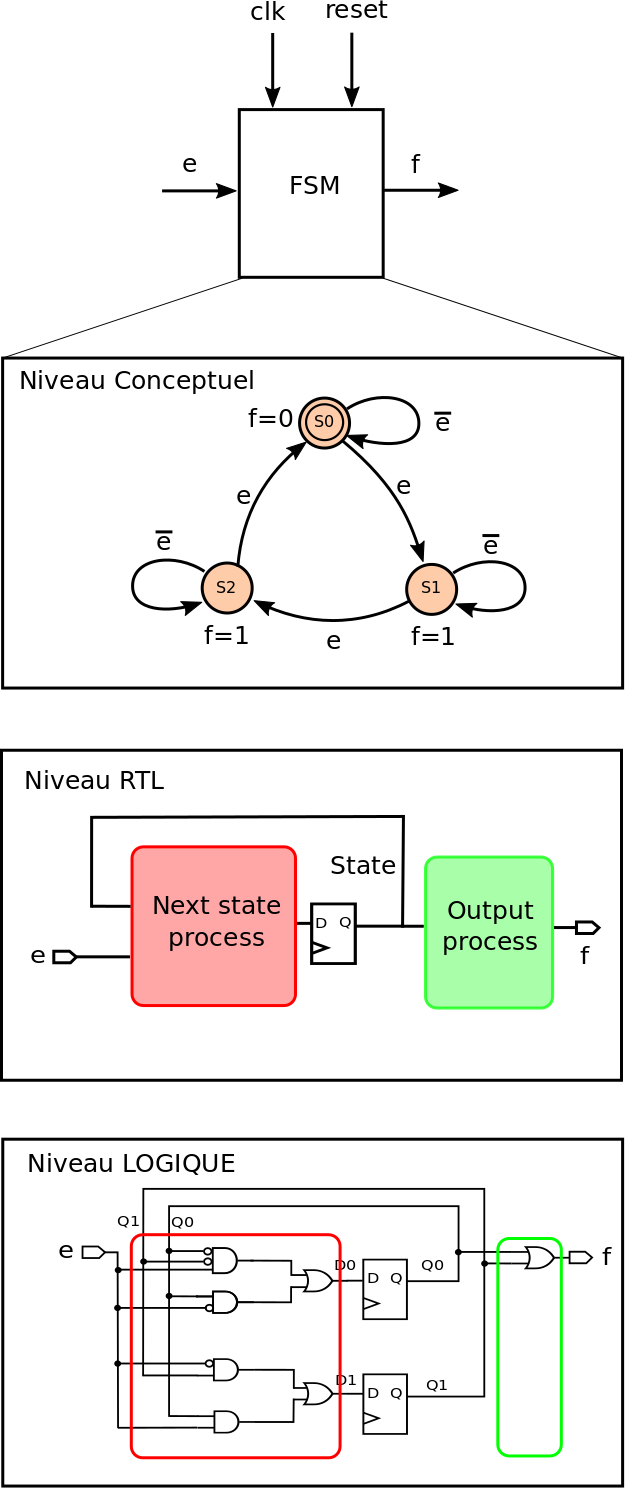
\includegraphics[width=6cm]{./figures/exo_fsm_expanded.png}
   \end{minipage}
\end{center} % added ending }

Cette description est plus longue que la précédente, mais ce n'est pas le cas en général. La description RTL est généralement plus concise et surtout beaucoup plus explicite.

Notons que l'entité n'a pas besoin d'être à nouveau déclarée : elle est commune aux deux architectures. Dit autrement : à cette entité correspondent deux architectures (ou réalisations) différentes.

\section{Simulation en VHDL}

Nous présentons ici un survol des premiers principes de simulation en VHDL. Bien évidemment, la simple édition et compilation d'un design VHDL ne garantit
pas le bon fonctionnement final du circuit : il est nécessaire de vérifier, à l'aide de ces simulations, que le comportement effectif du circuit, correspond
bien aux attentes du concepteur.

\subsection{Flot de conception général}

La simulation s'inscrit dans un {\it flot de conception} plus large. On utilise ce terme pour rendre compte de la succession d'étapes lors de la conception,
en partant des étapes amont, vers des étapes aval. Les grandes étapes de ce flot sont outillées et donnent lieu à des spécialisations de la part
des concepteurs : il est désormais impossible de maîtriser dans son ensemble les compétences nécessaires au bon déroulement de ce flot, essentiellement du fait
de la multiplicités des outils mis en jeu. Ce flot est illustré sur la figure suivante. La simulation correspond à la partie amont du flot, alors que la synthèse (RTL et logique, non séparées ici)
apparaît dans la partie aval.

\begin{center}
\begin{minipage}[t]{8cm}
 \centering
 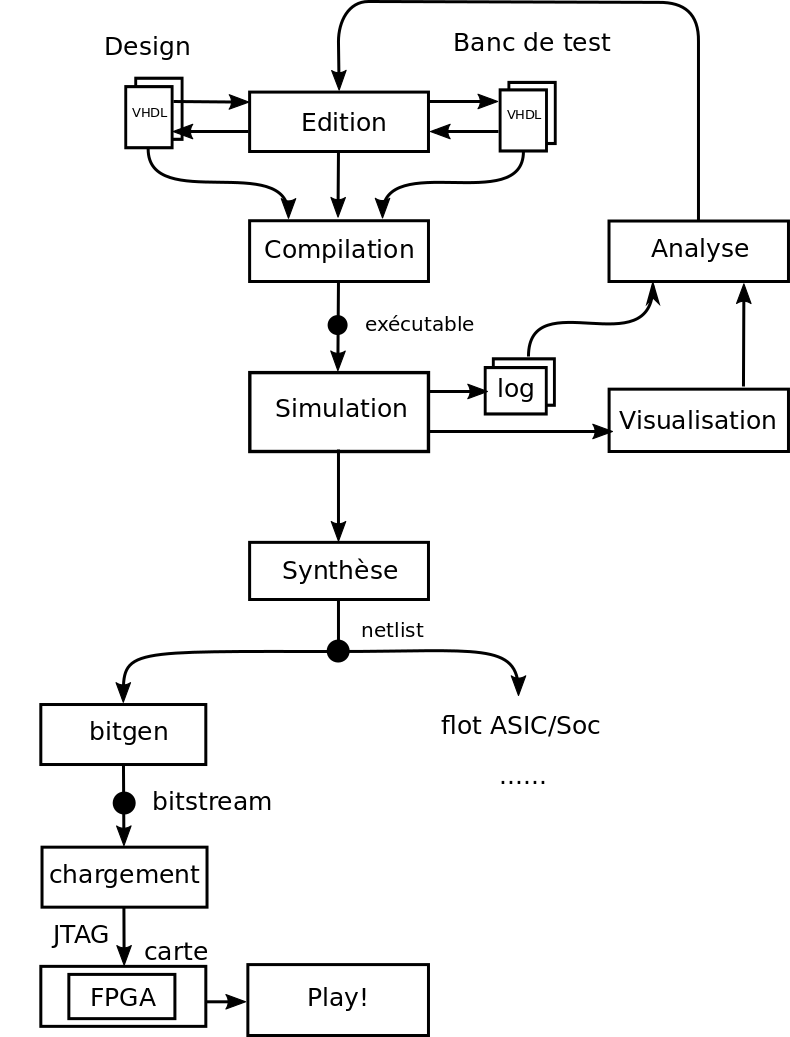
\includegraphics[width=8cm]{./figures/conception_generale.png}
\end{minipage}
\end{center}


\subsection{Bancs de tests ou {\it Testbench} pour la vérification}

Les bancs de tests VHDL (ou testbenches en anglais) permettent de se doter d'{\it instruments virtuels}, également décrits en VHDL.
Ces instruments, lorsqu'ils ne sont pas virtuels, coûtent chacun une petite fortune ! C'est l'intérêt de la simulation.
Ces instruments sont de deux types : générateurs de signaux, et analyseurs de signaux. De manière simplifiée, et en première approximation,
on peut considérer que chaque instrument revient à écrire un processus VHDL. Ces processus n'ont pas vocation à être traduits en portes logiques : ils
pourront bénéficier des facilités "logicielles" traditionnelles d'un langage moderne : boucle, procédures, fonctions, etc. sans avoir à se soucier
de leur "synthétisabilité".

\begin{figure}[!t]
  \centering
  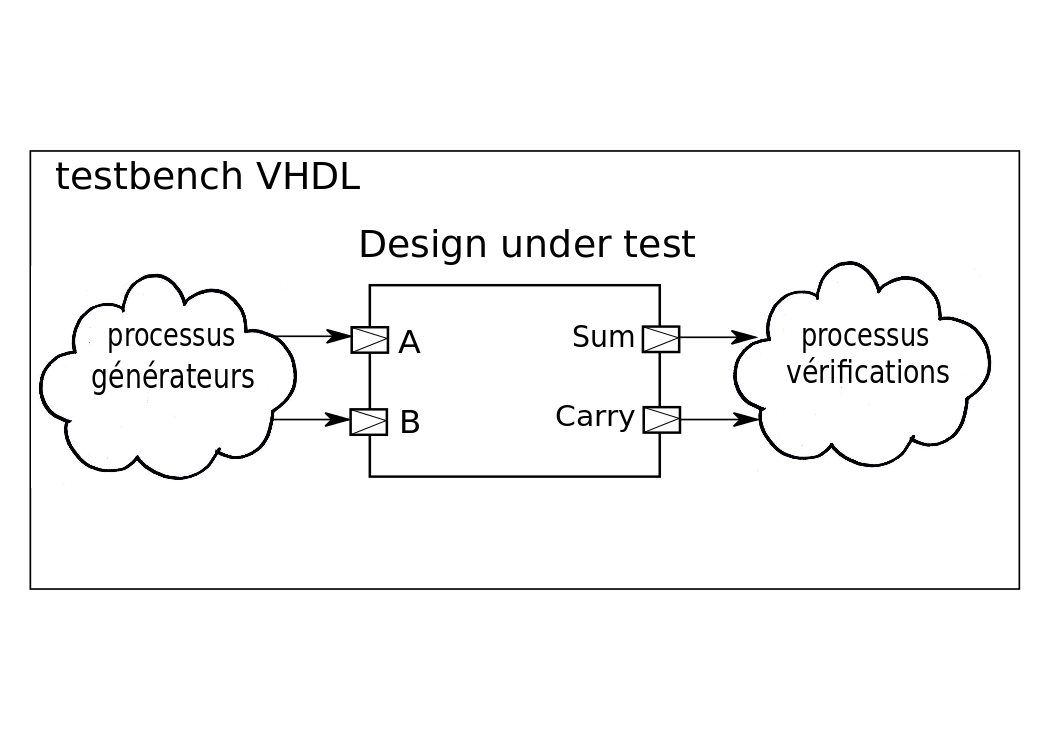
\includegraphics[width=8cm]{./figures/testbench.png}
  \caption{Idée de banc de test primitif : des processus excitent le circuit et observent ses réactions.}
  \label{tb}
\end{figure}

\paragraph{Génération de l'horloge}
A titre d'exemple, voici un générateur d'horloge simplissime : pour peu que le signal ait été initialisé, lors de sa déclaration, à une valeur 0 ou 1,
le signal "clk" change de valeur toute les demi-périodes d'horloge (la constante HALF\_PERIOD a été déclarée au préalable). Il est hors de question de
chercher à synthétiser ce signal matériellement : c'est un circuit combinatoire (inverseur) rebouclé sur lui-même, ce qui est proscrit des règles
de conception synchrone que l'on s'est fixées ! Mais, pour la simulation, ce signal fait l'affaire. Il représente bien un signal oscillant de 0 à 1 et de 1 à 0, parfaitement
périodique. Par contre, ce style de codage oblige souvent à arrêter la simulation de manière "sauvage" : sans un tel arrêt, la simulation continue ad vitam aeternam...

\begin{lstlisting}[frame=single]
 clk <= not(clk) after HALF_PERIOD;
\end{lstlisting}

On utilisera dans nos travaux pratiques un générateur d'horloge légèrement plus sophistiqué. Le code suivant permet de piloter la génération du signal, grâce
à une condition qui provient d'un signal booléen (true,false) "running". Ceci permet astucieusement de non seulement stopper l'horloge, mais par là-même de
ne plus générer un seul événement pour le simulateur : c'est une fin d'exécution {\it par famine}. Cela permet, au sein d'un banc de test, de décider le moment où le simulateur doit s'arrêter. Par exemple,
après avoir appliqué un ensemble de tests, executés par un processus, ce processus pilote le signal running à "false".

\begin{lstlisting}[frame=single]
 clk <= not(clk) after HALF_PERIOD when running else clk;

 stim : process
 begin
   -- long test...
   -- skipped...
   running <= false; --arret par famine
   wait;
 end process;
\end{lstlisting}

\subsection{Modèles de référence}
Le schéma \ref{tb} précédent n'illustre pas complètement la difficulté à réellement vérifier le bon fonctionnement du circuit. Vérifier un circuit
ne peut se pas se limiter à une simple "vérification visuelle" de la bonne forme de certains signaux : les designs sont généralement trop complexes pour
se contenter d'une une simple "opinion".
Il est nécessaire de développer des méthodologies qui permettent de {\it comparer} le comportement simulé avec un comportement supposé correct.
Le schéma suivant illustre à l'inverse le recours à un modèle supposé correct : il est d'usage d'appeler ce modèle un {\it golden model}. C'est un modèle
qu'on ne remettra pas en question lors de la vérification.

\begin{center}
\begin{minipage}[t]{8cm}
 \centering
 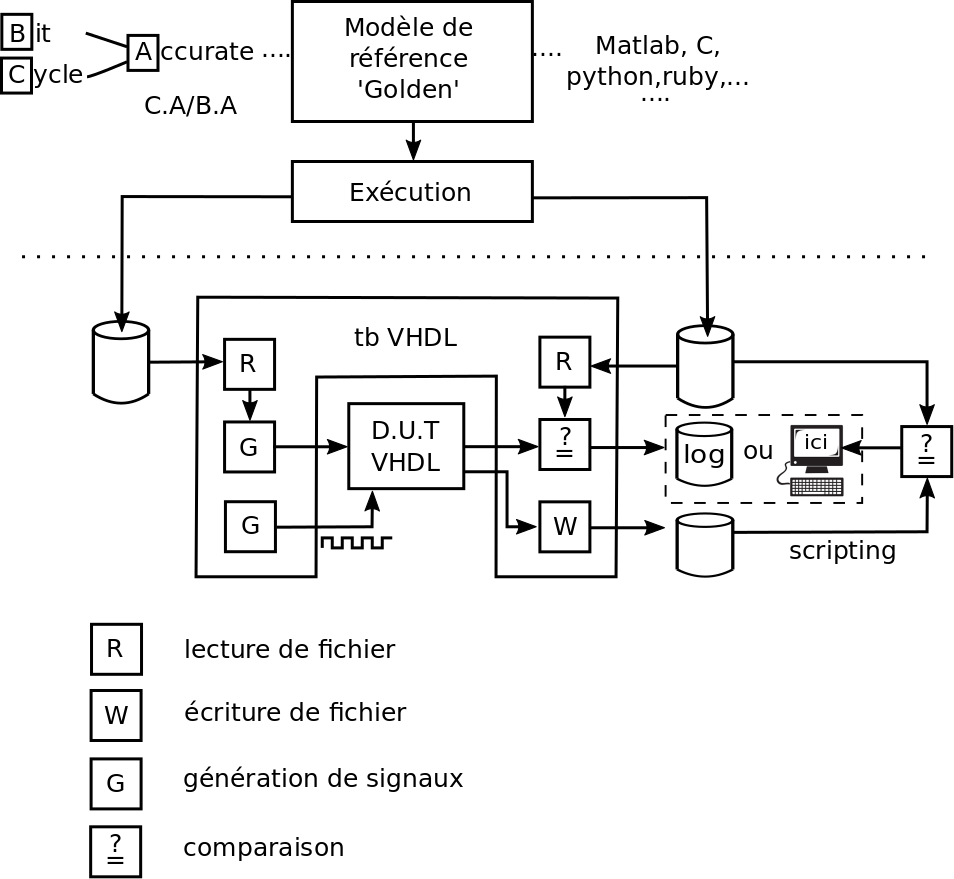
\includegraphics[width=10cm]{./figures/flot_testbench.png}
\end{minipage}
\end{center}

Ce modèle est issu le plus généralement d'équipes d'algorithmiciens. A l'issu de leur activité, il leur est possible
de mettre à disposition des fichiers d'entrées-sorties de leur algorithme. La difficulté est de s'entendre sur le contenu de
ces fichiers. Par exemple, les algorithmiciens n'ont pas la même perception du temps : il est rare qu'ils soient en mesure
de fournir des données de référence exacte au cycle près ({\it cycle-accurate models}). Le plus souvent les données
restent cependant précises au bit près ({\it bit-accurate models}). Toute sorte de modèles intermédiaires sont imaginables.

%=================================================================
\section{Fonctionnement interne d'un simulateur VHDL}
\paragraph{Idée de causalité}
Comment fonctionne un simulateur VHDL ? Nos équations logiques et nos structures séquentielles se présentent comme
un vaste enchevêtrement de signaux, interconnectés les uns aux autres, sans ordre évident.
Un simulateur de circuits doit simuler l'existence de phénomènes
temporels logico-physiques, qui se déroulent parfois les uns à la suite des autres, ou parfois de manière parallèle.
 Mais, dans tous les cas, le simulateur est un algorithme
qui s'exécute sur un PC, qui est essentiellement séquentiel : l'algorithme de simulation doit être en mesure de correctement restituer
l'idée de {\it causalité}. Le respect de la causalité est essentiel : notamment on comprend bien qu'une modification d'un signal à un temps $t$ ne peut
avoir de conséquence à un temps antérieur.

\paragraph{Simulateur à événements discrets}

L'algorithme le plus flexible pour accomplir cette prouesse s'appelle un {\it simulateur à événements discrets}. En VHDL,
un {\it événement} est un {\it changement de valeurs} d'un signal donné. Cet évenement est associé à un {\it timestamp}, c'est-à-dire
une information sur la date où doit survenir cet événement. Le travail du simulateur va donc être de gérer une vaste liste d'événements
planifiés. A partir d'une première collecte effectué au temps simulé $t=0$, un premier ensemble d'événements est enregistré.
Ce premier ensemble va agir par "effet d'avalanche" : ces événements vont déclencher de nouveaux événements au fur-et-à-mesure
de l'exécution du simulateur. Ces évenements "primitifs" proviennent d'une écriture spécifique utilisée
par le concepteur VHDL : il est par exemple possible en VHDL d'exprimer les modifications qu'un signal rencontrera au cours du temps. Ainsi le code
suivant indique que simulateur qu'à $t=0$ le signal $s$ prend la valeur $1$. Toutefois, il est d'ores-et-déjà enregistré que dans le futur, à $t=12 ns$,
 ce signal vaudra '0' etc.

\begin{lstlisting}[frame=single]
 s <= '1', '0' after 12 ns, '1' after 34 ns;
\end{lstlisting}

Cette première collecte  s'effectue sur l'ensemble du système numérique décrit. Au sein des processus VHDL,
cette évaluation s'arrête localement aux instructions "wait". Le processus continuera d'être évalué, au cours de la simulation,
 lorsque la condition du wait sera effectivement remplie. Lorsque l'évaluation atteint la fin d'un processus, le simulateur considère
 qu'il doit reprendre l'évaluation du processus à partir de son début.

 Au cours de la collecte, le simulateur a également analysé les listes de sensibilité des processus : il sait donc que tel
 processus, sensible à un signal $s$, devra être réévalué dès lors qu'un nouvel événement survient sur $s$.
A l'issue de cette première collecte, le simulateur cherche le timestamp $t$ le plus proche dans le futur.

Il exécute tous les processus sensibles à ce signal, ou les reprend au point d'exécution où il s'était précédemment arrêté.
C'est au cour de cette exécution que tout un ensemble de nouveaux événements sera planifié {\it dans le futur}.

\paragraph{Temps physique et délai delta}
L'ordonnancement des événements se fait non seulement sur le temps physique, mais également sur un temps appelé "delta", qui correspond
à un temps $\delta t$ infinitésimal. Ce temps est ajouté au timestamp d'un signal, lors de l'assignation de ce signal. Ce "delta delay"
permet de maintenir l'idée de précédence et de causalité au sein des affectations s'effectuant au même pas de temps physique.

\section{Utilisation du simulateur GHDL}


\subsection{Introduction}
GHDL est un simulateur open source développé par Tristan Gingold, un ingénieur français.
A la différence d'outils professionnels comme Modelsim de la société Mentor Graphics, GHDL s'utilise
uniquement en ligne de commande. GHDL peut être être utilisé en synergie avec un second outil appelé GTKWave dans le but de visualiser des chronogrammes.
Nous rappelons ici les commandes utiles qui permettent de simuler un circuit simple.
D'autres commandes sont disponibles mais ne seront pas traitées ici.

\subsection{Commandes essentielles}


GHDL s'utilise en ligne de commande comme n'importe quel compilateur.
Le 'G' de GHDL fait référence au projet GNU lié à l'Open source dont le fer de lance est GCC, le compilateur pour le langage C (et bien d'autres langages !).
D'ailleurs GHDL utilise le même backend que GCC : il génère les mêmes fichiers binaires "*.o". A la date de rédaction (2017), une version de GHDL génère un bitcode
LLVM, alternative à GCC.

Les options les plus utiles sont les suivantes, utilisée dans cet ordre :
\begin{itemize}
  \item \textbf{ghdl \-a nom\_fichier.vhd} : Analyse le fichier et génère un binaire (faites ls -a nom\_fichier.o pour le voir si vous le souhaitez). Généralement il faut compiler plusieurs fichiers avant de passer à l'étape suivante.
 \item \textbf{ghdl \-e nom\_de\_l'entité\_simulable}  : Elaboration (ou Edition de lien), qui crée le simulateur compilé : c'est un exécutable comme un autre. Il embarque un moteur de simulation à événement discret.
\item \textbf{ghdl \-r nom\_de\_l'entité\_simulable}  : Run de l'exécutable précédent. Il est tout à fait possible de lancer l'exécutable sans passer par cette commande.
\end{itemize}

Généralement, on cherche à enregistrer les formes d'ondes (waveforms ou chronogrammes) dans un fichier, pour une visualisation post-mortem (c'est un désavantage de ghdl par rapport à Modelsim, qui permet d'arrêter une simulation et de la reprendre etc). La manière de faire consiste à modifier la dernière commande précédente :

\begin{lstlisting}[language=bash]
 $ ghdl -r entite_simulable --wave=fichier.ghw}
\end{lstlisting}

Le fichier au format ghw est ensuite lisible par le logiciel Gtkwave.

\begin{lstlisting}[language=bash]
    $ gtkwave fichier.ghw
\end{lstlisting}

Le logiciel Gtkwave permet de naviguer dans la hiérarchie de votre design, et de sélectionner les signaux que vous souhaitez visualiser.
Cette sélection peut être enregistrée pour une visualisation future, en sauvant un fichier .sav (passer par le menu de gtkwave). On pourra alors
relancer la simulation en demandant à GTKWave d'afficher automatiquement ces signaux.

\begin{lstlisting}[language=bash]
  gtkwave fichier.ghw signaux.sav
\end{lstlisting}

Au final, il est possible d'automatiser le processus de compilation-simulation-visualisation en copiant les commandes précédentes dans un script.
N'oubliez pas de rendre ce script exécutable, en lui donnant les bons droits (chmod +x nom\_script).

\begin{center}
\begin{minipage}[t]{10cm}
 \centering
 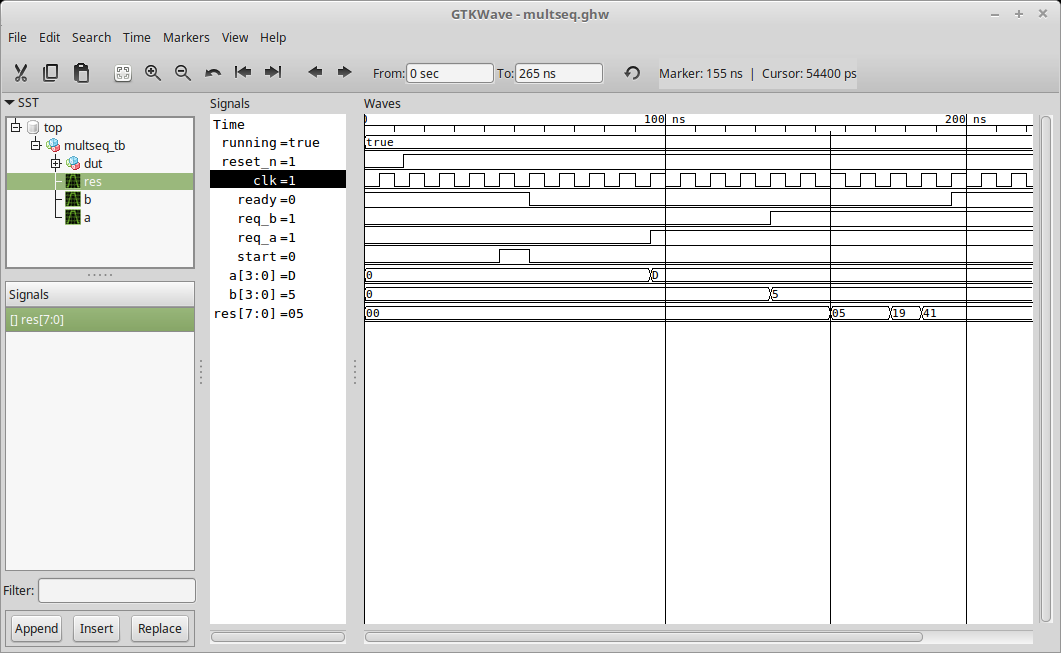
\includegraphics[width=10cm]{./figures/gtkwave.png}
\end{minipage}
\end{center}

\section{Conclusion}
Ce chapitre nous a permis d'aborder VHDL de manière simplifiée, et d'appréhender la difficulté de mettre au point un circuit un tant soit peu complexe.
La simulation requiert une forte discipline non seulement pour le concepteur, mais également pour un environnement d'ingénierie plus vaste encore, faisant
intervenir d'autres spécialistes. Nous avons cantonné la simulation au niveau logique et débordé sur le niveau RTL (concernant les automates). VHDL permet
d'aller plus loin dans la simulation , en simulant les délai des portes logiques en présence. VHDL permet également de remonter en abstraction : les bancs de
test illustrent cette remontée, puisqu'il est possible d'y utiliser des constructions de langage plus habituels dans un "langage traditionnel". Cette richesse
sera étudiée en deuxième année.\\

%On pourra compléter la lecture de cette introduction par la consulation du livre de Pong Chu \cite{Chu2008}.
